\documentclass[tikz,border=10pt]{standalone}
\usepackage{pgfplots}
\pgfplotsset{compat=1.16}

\begin{document}

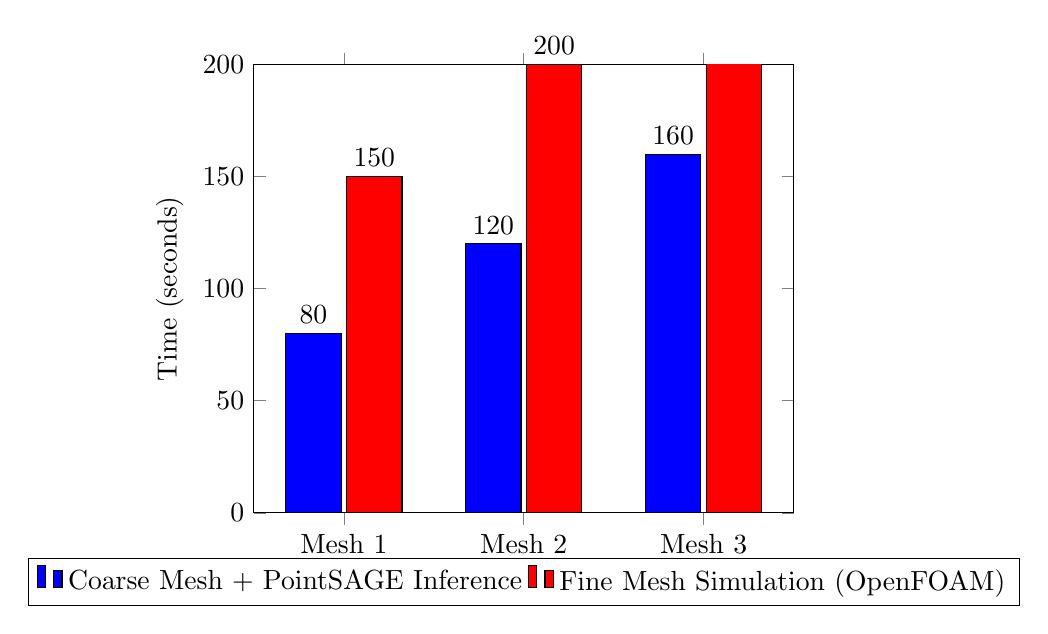
\begin{tikzpicture}
    \begin{axis}[
        ybar,
        symbolic x coords={Mesh 1, Mesh 2, Mesh 3},
        xtick=data,
        nodes near coords,
        nodes near coords align={vertical},
        ylabel={Time (seconds)},
        legend style={at={(0.5,-0.1)}, anchor=north,legend columns=-1},
        bar width=20pt,
        ymin=0,
        ymax=200,
        enlarge x limits=0.25
    ]
        \addplot[fill=blue] coordinates {(Mesh 1, 80) (Mesh 2, 120) (Mesh 3, 160)};
        \addlegendentry{Coarse Mesh + PointSAGE Inference}
        
        \addplot[fill=red] coordinates {(Mesh 1, 150) (Mesh 2, 200) (Mesh 3, 250)};
        \addlegendentry{Fine Mesh Simulation (OpenFOAM)}
    \end{axis}
\end{tikzpicture}

\end{document}